\documentclass{article}
\usepackage{ctex}
\usepackage{xltxtra}
\usepackage{graphicx}
\usepackage{xcolor}
\usepackage{amsmath}
\usepackage{subfigure}
\usepackage{geometry}
\usepackage{amssymb}
\usepackage{booktabs}
\geometry{a4paper,left=2cm,right=2cm,top=2cm,bottom=2cm}
\graphicspath{{../fig/}}

\title{{\bf Project2: Multigrid for Possion Equation}}
\author{陈震翔\\3210103924 信息与计算科学}

\date{}

\begin{document}

\maketitle

\section{理论分析}
\subsection{差分格式}
与Project1相同
\subsection{Quadratic interpolation on one Dimensions}
$v_{2j}^h = v_j^{2h},\ v_{2j+2}^h = v_{j+1}^{2h},\ v_{2j+4}^h = v_{j+2}^{2h}$

然后用$v_j^{2h},\ v_{j+1}^{2h},\ v_{j+2}^{2h}$三点对$v_{2j+1}^h,\ v_{2j+3}^h$进行插值

设这五个点分别为$x_0^{2h},\ x_1^{2h}=x_0^{2h}+2h,\ x_2^{2h}=x_0^{2h}+4h,\ x_0^h=x_0^{2h}+h,\ x_1^h=x_0^{2h}+3h$

利用牛顿插值可得$v_j^{2h},\ v_{j+1}^{2h},\ v_{j+2}^{2h}$三点的插值多项式为
$$p(x) = v_j^{2h}+\frac{v_{j+1}^{2h}-v_j^{2h}}{2h}(x-x_0^{2h})+\frac{v_j^{2h}-2v_{j+1}^{2h}+v_{j+2}^{2h}}{8h}(x-x_0^{2h})(x-x_1^{2h})$$

代入得$v_{2j+1}^h=\frac{3v_j^{2h}+6v_{j+1}^{2h}-v_{j+2}^{2h}}{8},\ v_{2j+3}^h=\frac{3v_{j+2}^{2h}+6v_{j+1}^{2h}-v_{j}^{2h}}{8}$
\subsection{Restriction and Prolongation on Two Dimensions}
\subsubsection{Restriction}
\begin{itemize}
    \item \textbf{Injection}: $$v_{i,j}^{2h} = v_{2i,2j}^{h}$$
    \item \textbf{Full Weighting}:
    \begin{align}
        v_{i,j}^{2h} = & \frac{1}{4}(v_{2i,2j}^{h} \notag \\
        &+\frac{1}{2}(v_{2i-1,2j}^{h}+v_{2i+1,2j}^{h}+v_{2i,2j-1}^{h}+v_{2i,2j+1}^{h}) \notag \\
        &+\frac{1}{4}(v_{2i-1,2j-1}^{h}+v_{2i+1,2j+1}^{h}+v_{2i+1,2j-1}^{h}+v_{2i-1,2j+1}^{h})) \notag
    \end{align}
    如下图
    \begin{figure}[h]
        \centering
        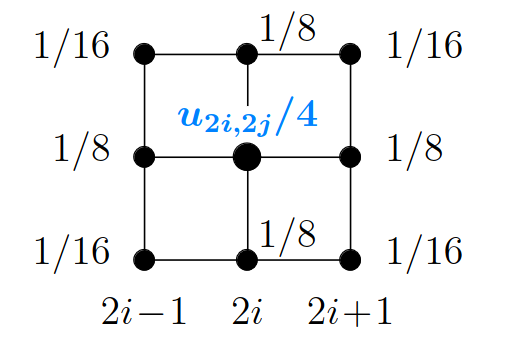
\includegraphics[width = 0.25\linewidth]{fw2D.png}
    \end{figure}

    对于边界采取一维的Full Weighting Restriction,四个角则直接Injection。
\end{itemize}
\subsubsection{Prolongation}
二维网格的二次插值太过繁琐并且从一维网格的实验结果中发现二次插值相比线性插值在精度方面完全没有可以识别的提升,所以本实验中二维多重网格仅实现了线性插值。
二维的线性插值采用$bilinear$的形式,如下:
\begin{align}
    & v_{2i,2j}^h = v_{i,j}^{2h} \notag \\
    & v_{2i+1,2j}^h=\frac{1}{2}(v_{i,j}^{2h}+v_{i+1,j}^{2h})\notag\\
    & v_{2i,2j+1}^h=\frac{1}{2}(v_{i,j}^{2h}+v_{i,j+1}^{2h})\notag\\
    & v_{2i+1,2j+1}^h=\frac{1}{4}(v_{i,j}^{2h}+v_{i,j+1}^{2h}+v_{i+1,j}^{2h}+v_{i+1,j+1}^{2h})\notag
\end{align}

\subsubsection{Relation with One Dimension Operator}
事实上,利用$Kronecker\ product\otimes$,二维上的这两个操作可以定义为
$$I_{h(2D)}^{2h} := I_h^{2h}\otimes I_h^{2h} $$
$$I_{2h(2D)}^{h}(2D) := I_{2h}^{h}\otimes I_{2h}^{h} $$

并且若$I_h^{2h}(2D)$为$Full Weighting$时,有$I_{h(2D)}^{2h}=\frac{1}{4}(I_{2h(2D)}^{h})^T$

由一维时$I_h^{2h}=\frac{1}{2}(I_{2h}^{h})^T$加上$Kronecker\ product$即可得到。

\subsection{Convergence of Two Dimension Multigrid Method}
考虑如下的model problem
$$
\begin{cases}
    -\Delta u=f\quad &\text{in}\ \Omega:=(0,1)^2\\
    u = 0 & \text{on}\ \partial \Omega
\end{cases}
$$

由讲义的第七章可知,其对应的差分方程为$A_{2D}U=F$

$A_{2D}$为二维离散laplace算子,$A_{2D} = I\otimes A +A\otimes I$,$A$为一维离散laplace算子

$A$的特征值为$\lambda_k = \frac{4}{h^2}\sin^2\frac{k\pi}{2n}$,对应的特征值为$\mathbf{w}_k=[\sin\frac{k\pi}{n},\sin\frac{2k\pi}{n},\cdots,\sin\frac{(n-1)k\pi}{n}]^T$

那么$A_{2D}$的特征值以及对应的特征向量为$\lambda_{ij}=\lambda_i+\lambda_j,\ \mathbf{W}_{ij}=\text{vec}(\mathbf{w}_i\mathbf{w}_j^T)=\mathbf{w}_i\otimes\mathbf{w}_j$

\subsubsection{Relaxation}
令$A_{2D} = D-L-U$,其中 $D = \frac{4}{h^2}I$

那么对应的weight Jacobi迭代矩阵
\begin{align}
    T_{\omega(2D)} &=(1-\omega)I+\omega D^{-1}(L+U) \notag \\
    & = I - \frac{\omega h^2}{4}D + \frac{\omega h^2}{4}(L+U) \notag \\
    & = I - \frac{\omega h^2}{4}A_{2D} \notag
\end{align}

其特征向量与$A_{2D}$相同,对应的特征值为$$\lambda_{ij}(T_{\omega (2D)})=1-\lambda_{ij}= 1 - \omega\sin^2\frac{i\pi}{2n} -\omega\sin^2\frac{j\pi}{2n}$$

\subsubsection{Two-grid correction}
对于作用在误差向量上的二维Two-grid correction格式的迭代矩阵同一维的一致,为
$$TG_{(2D)}= T_{\omega(2D)}^{\nu_2}[I-I_{2h(2D)}^h(A_{(2D)}^{2h})^{-1}I_{h(2D)}^{2h}A_{(2D)}^h]T_{\omega(2D)}^{\nu_1}$$

\subsubsection{The spectral picture}
令$c_i = \cos^2\frac{i\pi}{2n},\ s_i = \sin^2\frac{i\pi}{2n},\ i'=n-i,\ j'=n-j$

\begin{itemize}
    \item Full Weighting Operator:
    \begin{align}
        I_{h(2D)}^{2h}\mathbf{W}_{ij}^h
        & = (I_{h}^{2h}\otimes I_{h}^{2h})(\mathbf{w}_i^h\otimes\mathbf{w}_j^h) \notag \\
        & = (I_{h}^{2h}\mathbf{w}_i^h)\otimes(I_{h}^{2h}\mathbf{w}_j^h) \notag \\
        & = (c_i\mathbf{w}_i^{2h})\otimes(c_j\mathbf{w}_j^{2h}) \notag \\
        & = c_ic_j(\mathbf{w}_i^{2h}\otimes\mathbf{w}_j^{2h}) \notag \\
        & = c_ic_j\mathbf{W}_{ij}^{2h} \notag
    \end{align}
    同理有$I_{h(2D)}^{2h}\mathbf{W}_{i'j}^h = -s_ic_j\mathbf{W}_{ij}^{2h},\ I_{h(2D)}^{2h}\mathbf{W}_{ij'}^h = -c_is_j\mathbf{W}_{ij}^{2h},\ I_{h(2D)}^{2h}\mathbf{W}_{i'j'}^h = s_is_j\mathbf{W}_{ij}^{2h}$
    \item Linear Interpolation Operator:
    \begin{align}
        I_{2h(2D)}^h\mathbf{W}_{ij}^{2h}
        & = (I_{2h}^{h}\otimes I_{2h}^{h})(\mathbf{w}_i^{2h}\otimes\mathbf{w}_j^{2h}) \notag \\
        & = (I_{2h}^{h}\mathbf{w}_i^{2h})\otimes(I_{2h}^{h}\mathbf{w}_j^{2h}) \notag \\
        & = (c_i\mathbf{w}_i^{h}-s_i\mathbf{w}_{i'}^{h})\otimes(c_j\mathbf{w}_j^{h}-s_j\mathbf{w}_{j'}^{h}) \notag \\
        & = c_ic_j(\mathbf{w}_i^{h}\otimes\mathbf{w}_j^{h})-s_ic_j(\mathbf{w}_{i'}^{h}\otimes\mathbf{w}_j^{h})-c_is_j(\mathbf{w}_{i}^{h}\otimes\mathbf{w}_{j'}^{h})+s_is_j(\mathbf{w}_{i'}^{h}\otimes\mathbf{w}_{j'}^{h}) \notag \\
        & = c_ic_j\mathbf{W}_{ij}^h-s_ic_j\mathbf{W}_{i'j}^h-c_is_j\mathbf{W}_{ij'}^h+s_is_j\mathbf{W}_{i'j'}^h \notag 
    \end{align}
\end{itemize}

接下来同讲义中类似证明$\text{span}\{\mathbf{W}_{ij}^h,\mathbf{W}_{i'j}^h,\mathbf{W}_{ij'}^h,\mathbf{W}_{i'j'}^h\}$是$TG_{(2D)}$的不变子空间

首先考虑$\nu_1=\nu_2=0$的情况
\begin{align}
                & A_{(2D)}^h\mathbf{W}_{ij}^h = \frac{4(s_i+s_j)}{h^2}\mathbf{W}_{ij}^h \notag \\
    \Rightarrow & I_{h(2D)}^{2h}A_{(2D)}^h\mathbf{W}_{ij}^h=\frac{4c_ic_j(s_i+s_j)}{h^2}\mathbf{W}_{ij}^{2h} \notag \\
    \Rightarrow & (A_{(2D)}^{2h})^{-1}I_{h(2D)}^{2h}A_{(2D)}^h\mathbf{W}_{ij}^h = \frac{4c_ic_j(s_i+s_j)}{h^2} \frac{(2h)^2}{4(4c_is_i+4c_js_j)}\mathbf{W}_{ij}^{2h} = \frac{c_is_ic_j+c_js_jc_i}{c_is_i+c_js_j}\mathbf{W}_{ij}^{2h} \notag \\
    \Rightarrow & -I_{2h(2D)}^h(A_{(2D)}^{2h})^{-1}I_{h(2D)}^{2h}A_{(2D)}^h\mathbf{W}_{ij}^h \notag \\
    & = -\frac{c_is_ic_j+c_js_jc_i}{c_is_i+c_js_j}(c_ic_j\mathbf{W}_{ij}^h-s_ic_j\mathbf{W}_{i'j}^h-c_is_j\mathbf{W}_{ij'}^h+s_is_j\mathbf{W}_{i'j'}^h) \notag \\
    & := -C_1\mathbf{W}_{ij}^h+C_2\mathbf{W}_{i'j}^h + C_3\mathbf{W}_{ij'}^h - C_4\mathbf{W}_{i'j'}^h \notag \\
    \Rightarrow & [I-I_{2h(2D)}^h(A_{(2D)}^{2h})^{-1}I_{h(2D)}^{2h}A_{(2D)}^h]\mathbf{W}_{ij}^h = (1-C_{11})\mathbf{W}_{ij}^h+C_{12}\mathbf{W}_{i'j}^h + C_{13}\mathbf{W}_{ij'}^h - C_{14}\mathbf{W}_{i'j'}^h\notag
\end{align}

因为$\forall i,\ 0 < ci,si < 1$,所以$0 < \frac{c_is_ic_j+c_js_jc_i}{c_is_i+c_js_j} < 1 \Rightarrow 0 < C_{1k} < 1$

所以$\mathbf{W}_{ij}^h,\mathbf{W}_{i'j}^h,\mathbf{W}_{ij'}^h,\mathbf{W}_{i'j'}^h$的系数的绝对值都小于1

再加上pre-smoothing和post-smoothing就有
$$TG_{(2D)}\mathbf{W}_{ij}^h=\lambda_{ij}^{\nu_1+\nu_2}(1-C_{11})\mathbf{W}_{ij}^h+\lambda_{ij}^{\nu_1}\lambda_{i'j}^{\nu_2}C_{12}\mathbf{W}_{i'j}^h + \lambda_{ij}^{\nu_1}\lambda_{ij,}^{\nu_2}C_{13}\mathbf{W}_{ij'}^h - \lambda_{ij}^{\nu_1}\lambda_{i'j'}^{\nu_2}C_{14}\mathbf{W}_{i'j'}^h$$

其中$\lambda_{ij}$为$T_{\omega(2D)}$的特征值,有$0 < \lambda_{ij} < 1$

所以上式中$\mathbf{W}_{ij}^h,\mathbf{W}_{i'j}^h,\mathbf{W}_{ij'}^h,\mathbf{W}_{i'j'}^h$的系数的绝对值都小于1

同理可知$TG_{(2D)}\mathbf{W}_{i'j}^h,\ TG_{(2D)}\mathbf{W}_{ij'}^h,\ TG_{(2D)}\mathbf{W}_{i'j'}^h$中$\mathbf{W}_{ij}^h,\mathbf{W}_{i'j}^h,\mathbf{W}_{ij'}^h,\mathbf{W}_{i'j'}^h$的系数的绝对值都小于1

所以对于二维的model problem,多重网格是收敛的

\subsection{How to analyse the reduction rate of V-cycle}
将残差看成一个迭代序列$\{\mathbf{r}_n\}$,显然当多重网格是收敛的时$$\lim_{n\rightarrow \infty} \mathbf{r}_n=0$$

若
$$\lim_{n\rightarrow \infty}\frac{|\mathbf{r}_{n+1}|}{|\mathbf{r}_n|^{\alpha}} = c$$

$\alpha$为收敛阶(本次实验中都为1),那么这里定义asymptotic factor $c$为reduction rate

\section{数值实验}
\subsection{概述}
\begin{itemize}
    \item 编写相应的程序
    \item 对不同的restriction、prolongation和cycle的组合求解如下六个方程
    
    1D:
    \begin{align}
        &\begin{cases}
            -u''(x) = (\sin(x)-(1+\cos(x))^2)e^{x+\sin(x)} \\
            u(x)|_{\Gamma} = e^{x+\sin(x)}\\
            u'(x)|_{\Gamma} = (1+\cos(x))*e^{x+\sin(x)} 
        \end{cases}\notag \\
        &\begin{cases}
            -u''(x) = \pi^2\sin(\pi x) \\
            u(x)|_{\Gamma} = \sin(\pi x)\\
            u'(x)|_{\Gamma}= \pi \cos(\pi x) 
        \end{cases}\notag \\
        &\begin{cases}
            -u''(x) = -6x \\
            u(x)|_{\Gamma} = x^3\\
            u'(x)|_{\Gamma} = 3x^2
        \end{cases}\notag
    \end{align}

    2D:
    \begin{align}
        &\begin{cases}
            -\Delta u(x,y) = (\sin(x)-\cos^2(x)-1)e^{y+\sin(x)} \\
            u(x,y)|_{\Gamma} = e^{y+\sin(x)}\\
            \frac{\partial u}{\partial n}|_{\Gamma} = \mathbf{n}\cdot \nabla e^{y+\sin(x)} 
        \end{cases}\notag \\
        &\begin{cases}
            -\Delta u(x,y) = 2\pi^2\sin(\pi x)\sin(\pi y) \\
            u(x,y)|_{\Gamma} = \sin(\pi x)\sin(\pi y)\\
            \frac{\partial u}{\partial n}|_{\Gamma} = \mathbf{n}\cdot \nabla \sin(\pi x)\sin(\pi y) 
        \end{cases}\notag \\
        &\begin{cases}
            -\Delta u(x,y) = -6(x+y) \\
            u(x,y)|_{\Gamma} = x^3+y^3\\
            \frac{\partial u}{\partial n}|_{\Gamma} = \mathbf{n}\cdot \nabla (x^3+y^3) 
        \end{cases}\notag
    \end{align}
        
    \item 边界条件:一维为左Neumann右Dirichlet; 二维为左边界和下边界为Neumann,右边界和上边界为Dirichlet。
    
    ps:对于纯Neumann边界的离散方程的系数矩阵奇异,无法求解,解决方案为一维只能求解纯Dirichlet条件和混合边界条件,二维指定四个角为真实值,近似为纯Neumann条件(对于直接法其实只用指定一个角为真实值即可,对于迭代法只指定一个角仍不收敛,为方便起见将四个角都设置为真实值)。
    \item 预设精度$\epsilon=10^{-8}$,最大迭代次数为100
    \item 求解后将结果输出到文件,包含各个粗细的网格上的数值解,误差,误差的最大模范数,求解时间,每次cycle后剩下的残差残差。
    文件编号说明, 1/2Dtest1/2/3对应一维和二维各三个测试方程,n=x为网格大小,Fwt/Inj(Full Weighting/Injection)、L/Q(Linear/Quadratic)、FMG/VC(Full Multigrid/V-cycle)、E/U/ErrorNorm/Time/Res(误差绝对值/数值解/误差范数/耗时/残差,同一个文件上不同网格的数据按从粗到细的顺序存储)。
    \item 将误差,误差的最大模范数,求解时间,每次cycle后剩下的残差残差绘制图像。
    \item 一维的误差绘制成函数图像,二维的误差绘制成热力图,同Project1相同,在不同粗细的网格上的误差分布相同,所以误差只展示最细网格的图像。
    \item 对误差的最大模范数,求解时间取$\log$绘制随$\log n$变化的图像,通过斜率判断收敛阶与时间复杂度
    \item 对数据分析后判断残差都是线性收敛的,绘制$\frac{|\mathbf{r}_{n+1}|}{|\mathbf{r}}$的图像,通过最后稳定的值判断reduction rate。
    \item 同时将各测试的耗时和迭代次数以及直接法LU分解的耗时输出到命令行,预设精度的测试结果也直接输出到命令行。
\end{itemize}
\subsection{实验结果}
\subsubsection{1D: $u(x)=e^{x+\sin(x)}$}
真实值:
\begin{figure}[h]
    \centering
    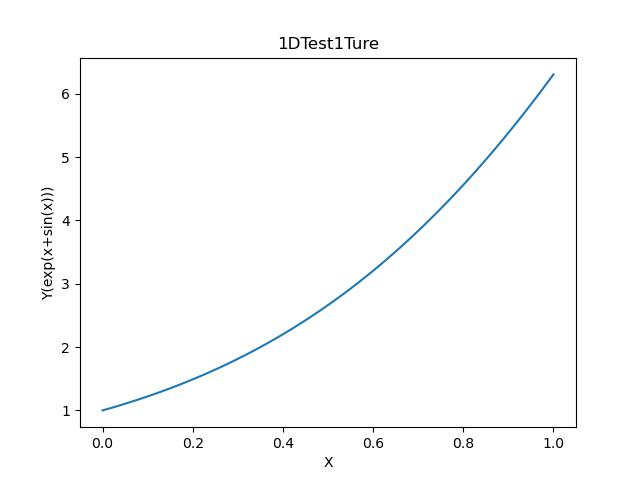
\includegraphics[width=0.7\linewidth]{1DTest1Ture.jpg}
\end{figure}
\newpage
\begin{itemize}
    \item Full Weighting, FMG, Linear
    \begin{figure}[h]
        \centering
        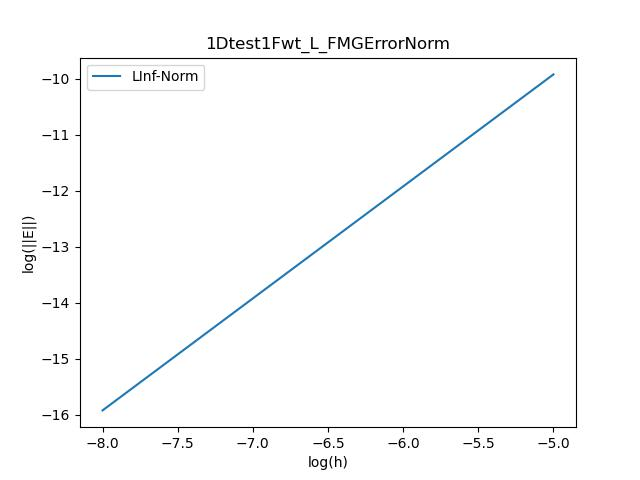
\includegraphics[width=0.35\linewidth]{1Dtest1Fwt_L_FMGErrorNorm.jpg}
        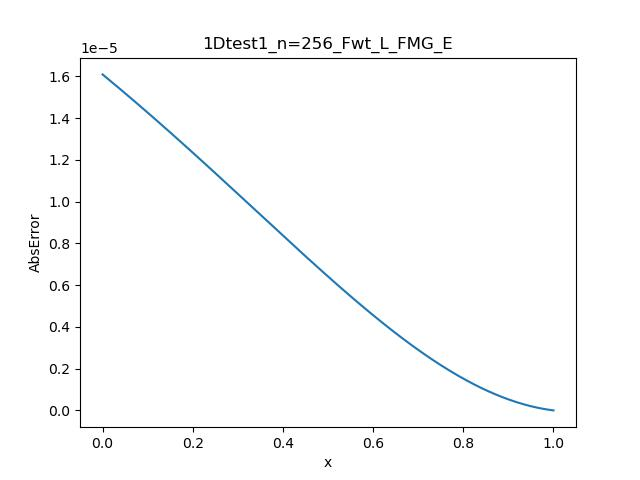
\includegraphics[width=0.35\linewidth]{1Dtest1_n=256_Fwt_L_FMG_E.jpg}
        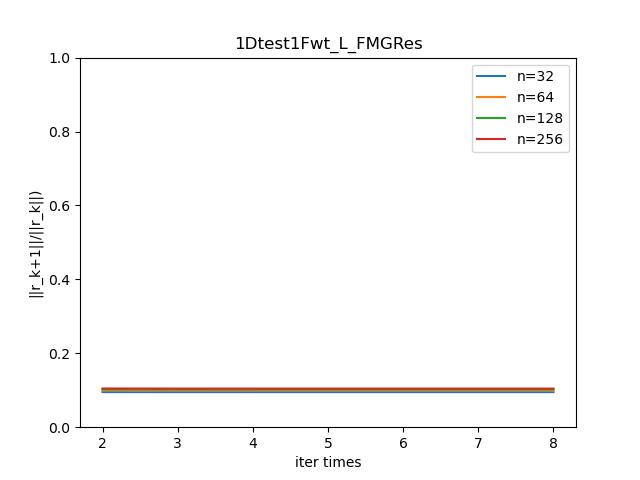
\includegraphics[width=0.35\linewidth]{1Dtest1Fwt_L_FMGRes.jpg}
        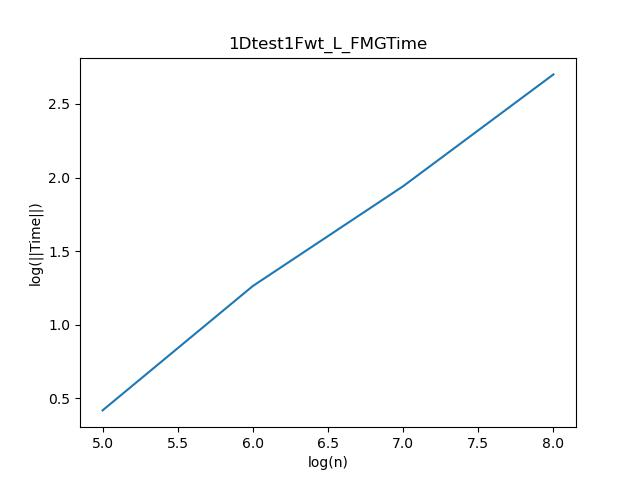
\includegraphics[width=0.35\linewidth]{1Dtest1Fwt_L_FMGTime.jpg}
    \end{figure}
    
    从图像可以判断收敛阶为2,残差的reduction rate 约为 0.1(即每迭代一次残差变为原先的0.1倍,下同), 时间复杂度为$O(n)$

    \item Injection, FMG, Linear
    \begin{figure}[h]
        \centering
        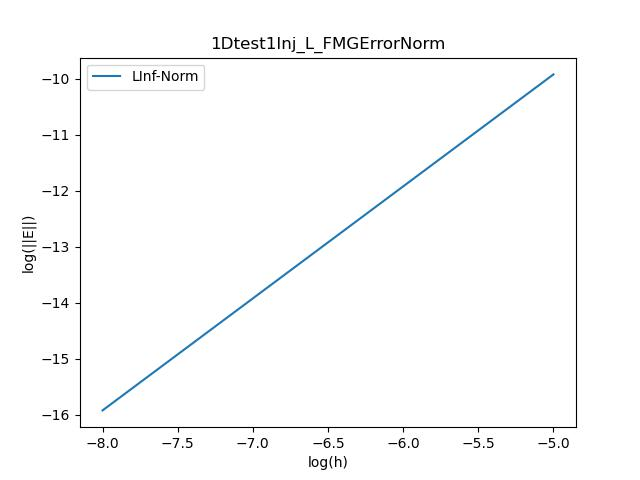
\includegraphics[width=0.35\linewidth]{1Dtest1Inj_L_FMGErrorNorm.jpg}
        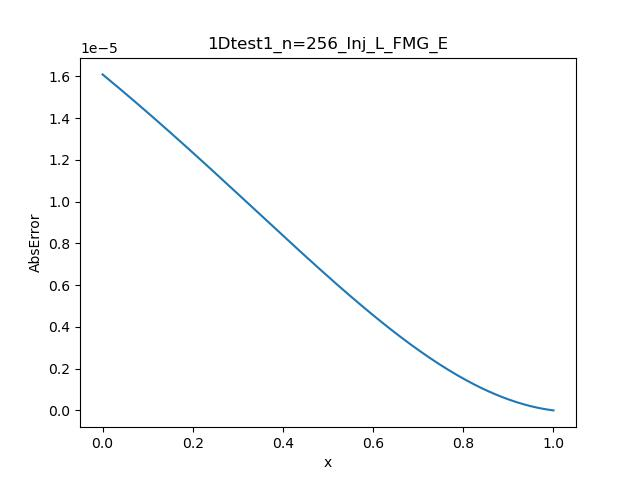
\includegraphics[width=0.35\linewidth]{1Dtest1_n=256_Inj_L_FMG_E.jpg}
        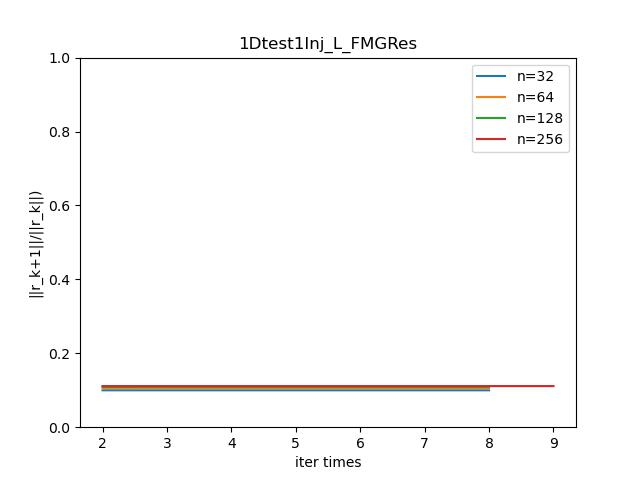
\includegraphics[width=0.35\linewidth]{1Dtest1Inj_L_FMGRes.jpg}
        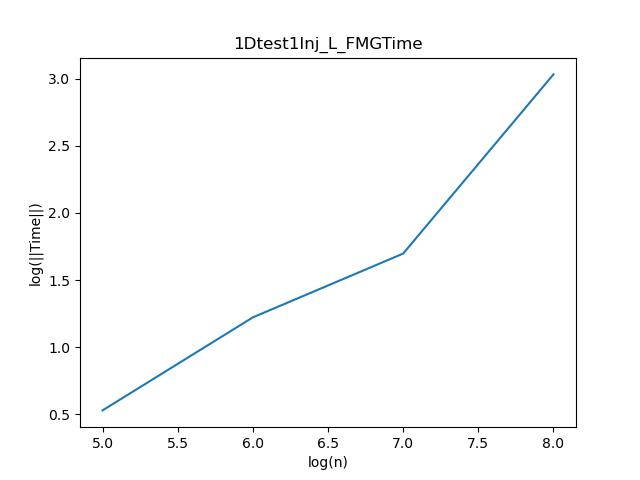
\includegraphics[width=0.35\linewidth]{1Dtest1Inj_L_FMGTime.jpg}
    \end{figure}
    
    从图像可以判断收敛阶为2,残差的reduction rate 约为 0.1, 时间复杂度为$O(n)$
    \newpage

    \item Full Weighting, VC, Linear
    \begin{figure}[h]
        \centering
        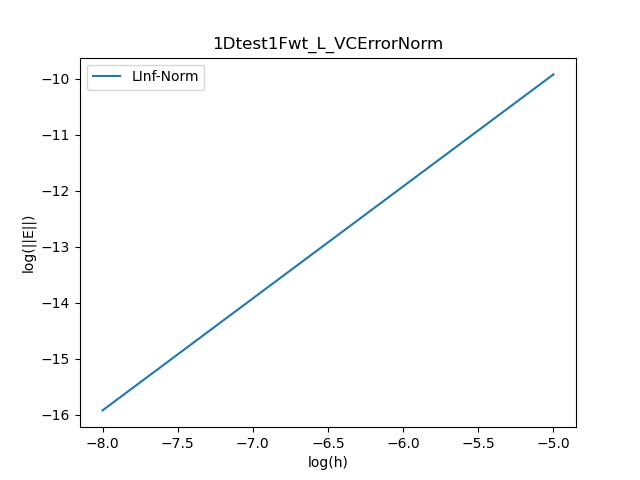
\includegraphics[width=0.35\linewidth]{1Dtest1Fwt_L_VCErrorNorm.jpg}
        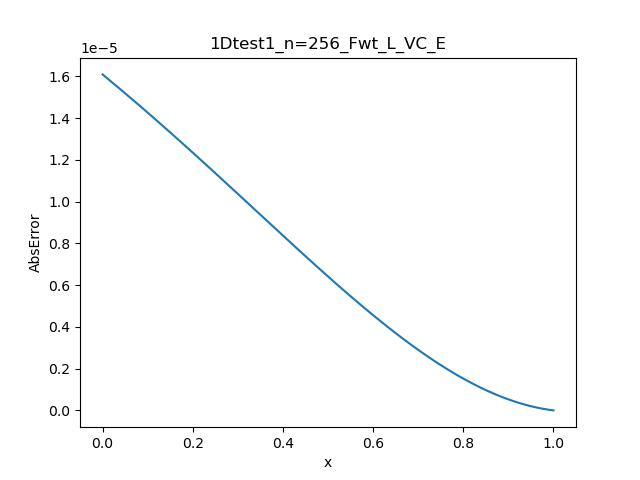
\includegraphics[width=0.35\linewidth]{1Dtest1_n=256_Fwt_L_VC_E.jpg}
        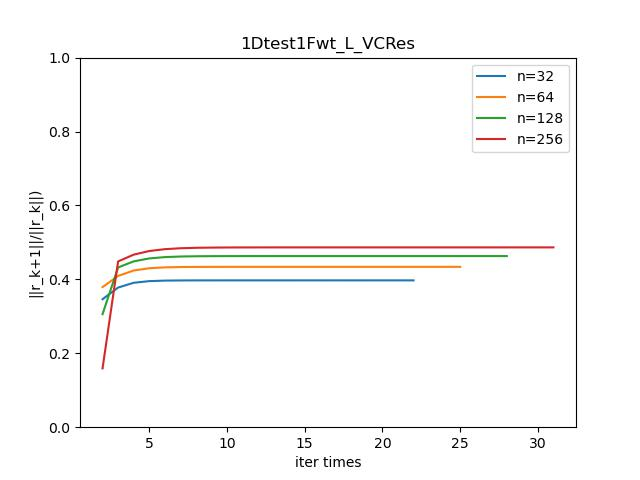
\includegraphics[width=0.35\linewidth]{1Dtest1Fwt_L_VCRes.jpg}
        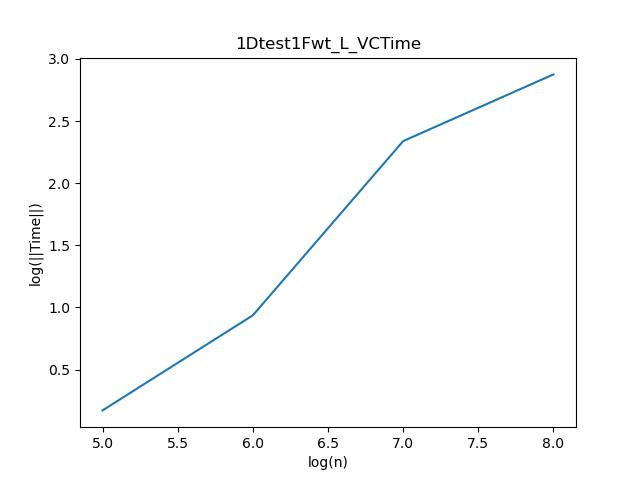
\includegraphics[width=0.35\linewidth]{1Dtest1Fwt_L_VCTime.jpg}
    \end{figure}
    
    从图像可以判断收敛阶为2,残差的reduction rate 随网格变细从约为0.35变化到约为0.45, 时间复杂度为$O(n)$

    \item Injection, VC, Linear
    \begin{figure}[h]
        \centering
        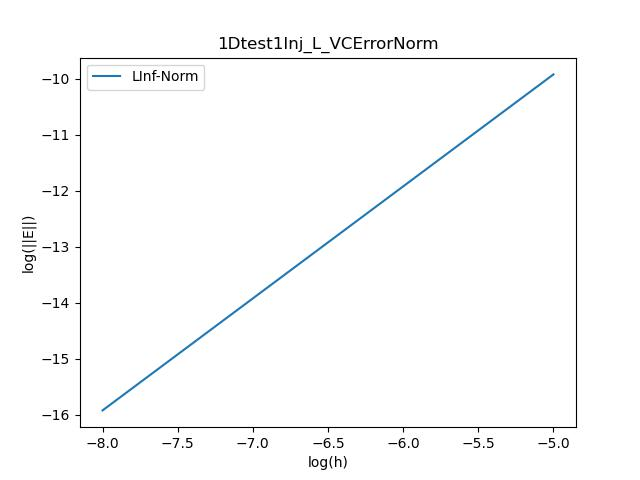
\includegraphics[width=0.35\linewidth]{1Dtest1Inj_L_VCErrorNorm.jpg}
        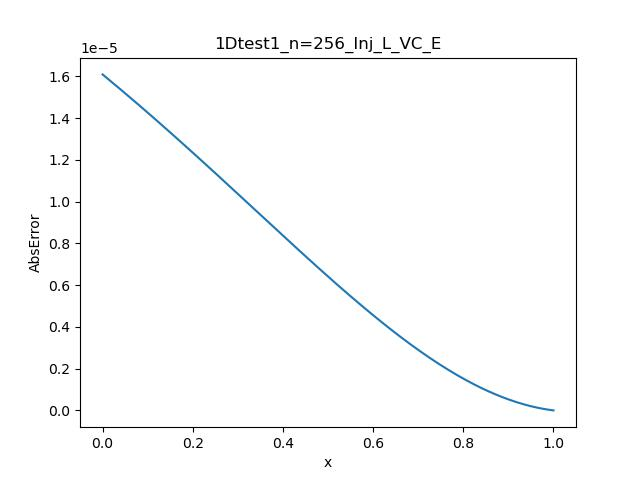
\includegraphics[width=0.35\linewidth]{1Dtest1_n=256_Inj_L_VC_E.jpg}
        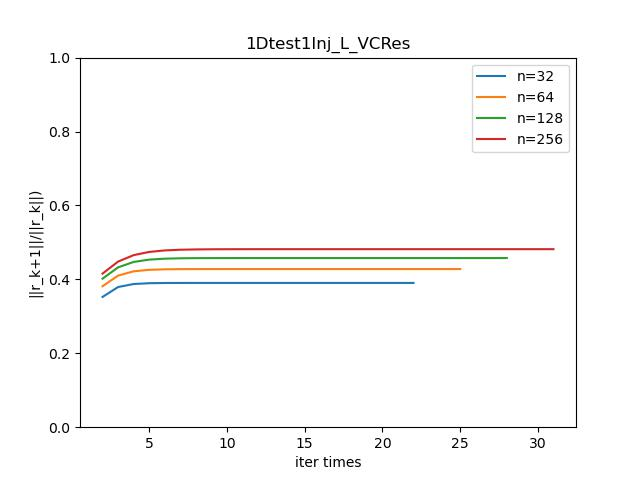
\includegraphics[width=0.35\linewidth]{1Dtest1Inj_L_VCRes.jpg}
        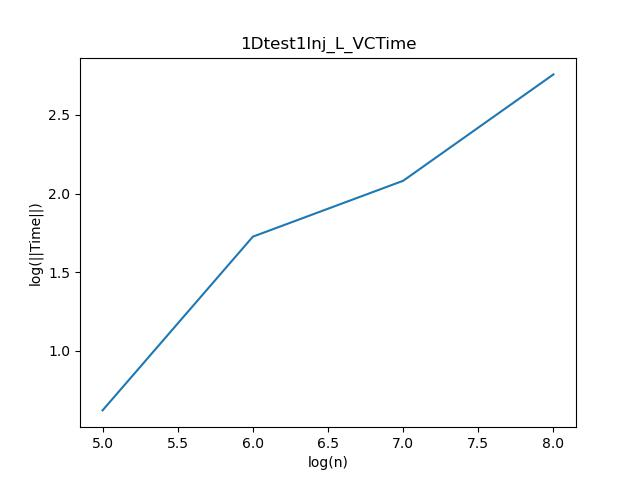
\includegraphics[width=0.35\linewidth]{1Dtest1Inj_L_VCTime.jpg}
    \end{figure}
    
    从图像可以判断收敛阶为2,残差的reduction rate随网格变细从约为0.35变化到约为0.45, 时间复杂度为$O(n)$
    \newpage
    \item Full Weighting, FMG, Quadratic
    \begin{figure}[h]
        \centering
        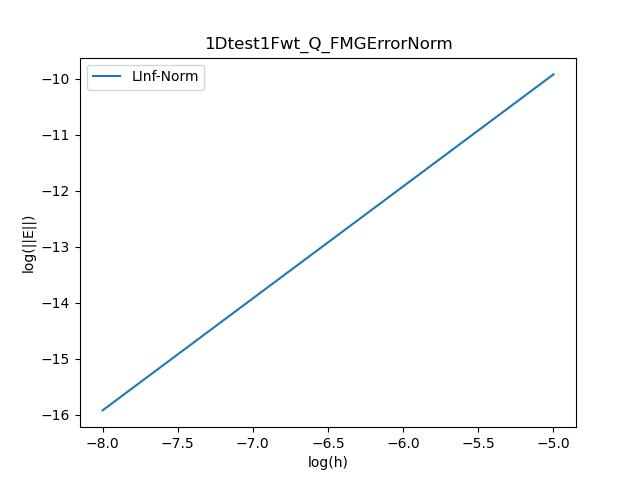
\includegraphics[width=0.35\linewidth]{1Dtest1Fwt_Q_FMGErrorNorm.jpg}
        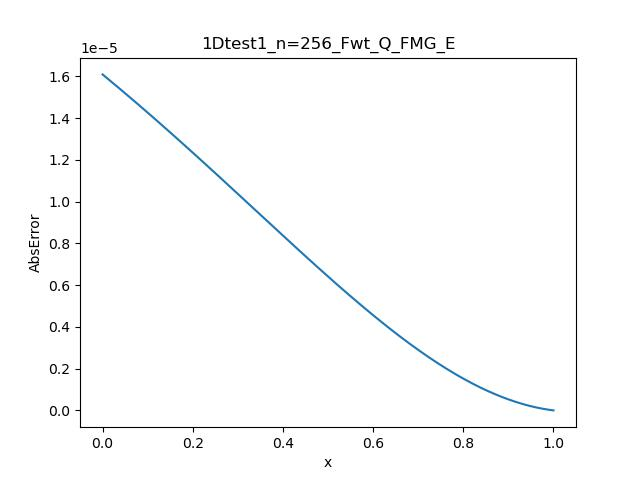
\includegraphics[width=0.35\linewidth]{1Dtest1_n=256_Fwt_Q_FMG_E.jpg}
        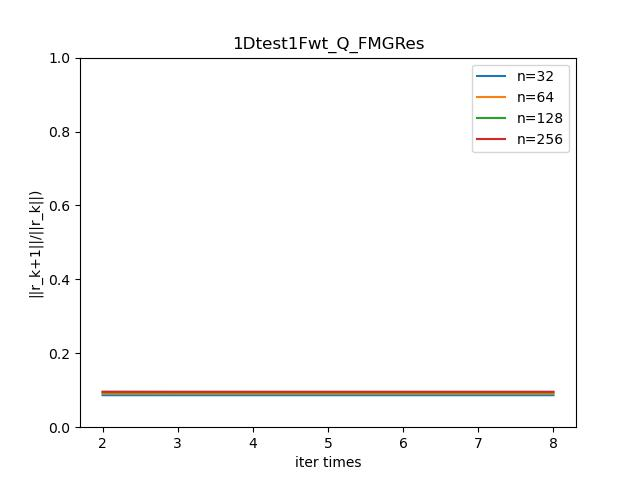
\includegraphics[width=0.35\linewidth]{1Dtest1Fwt_Q_FMGRes.jpg}
        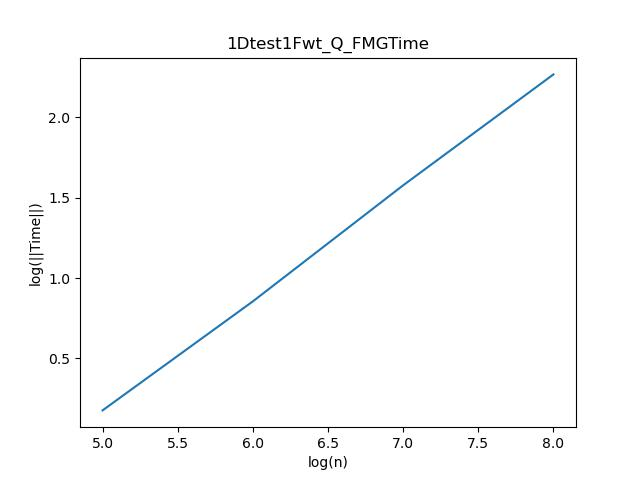
\includegraphics[width=0.35\linewidth]{1Dtest1Fwt_Q_FMGTime.jpg}
    \end{figure}
    
    从图像可以判断收敛阶为2,残差的reduction rate 约为 0.1, 时间复杂度为$O(n)$

    \item Injection, FMG, Quadratic
    \begin{figure}[h]
        \centering
        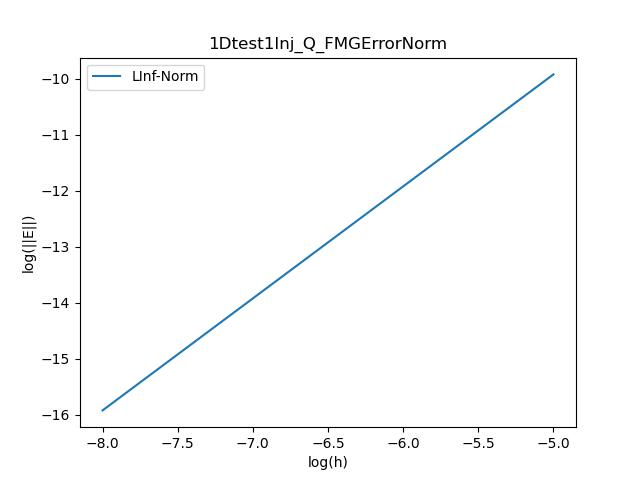
\includegraphics[width=0.35\linewidth]{1Dtest1Inj_Q_FMGErrorNorm.jpg}
        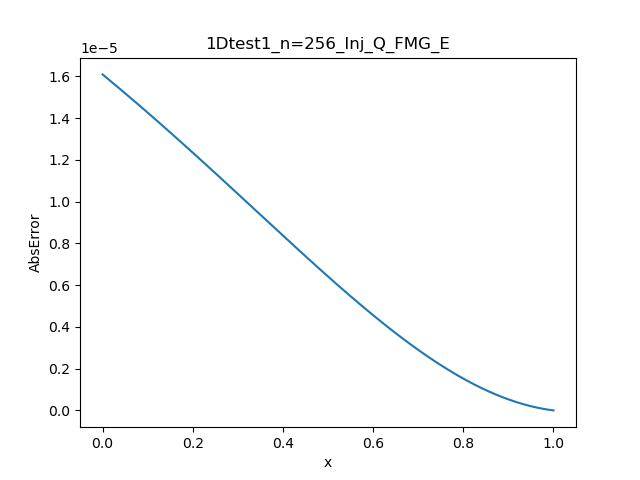
\includegraphics[width=0.35\linewidth]{1Dtest1_n=256_Inj_Q_FMG_E.jpg}
        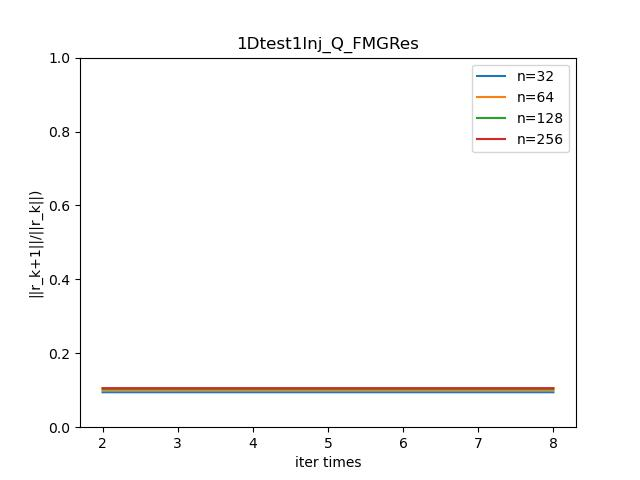
\includegraphics[width=0.35\linewidth]{1Dtest1Inj_Q_FMGRes.jpg}
        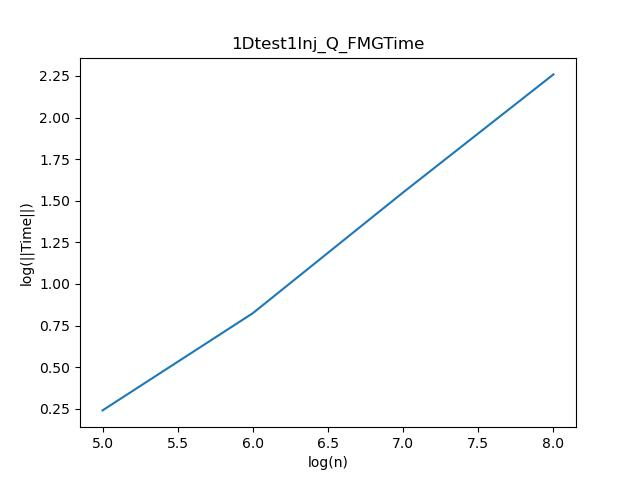
\includegraphics[width=0.35\linewidth]{1Dtest1Inj_Q_FMGTime.jpg}
    \end{figure}
    
    从图像可以判断收敛阶为2,残差的reduction rate 约为 0.1, 时间复杂度为$O(n)$
    \newpage

    \item Full Weighting, VC, Quadratic
    \begin{figure}[h]
        \centering
        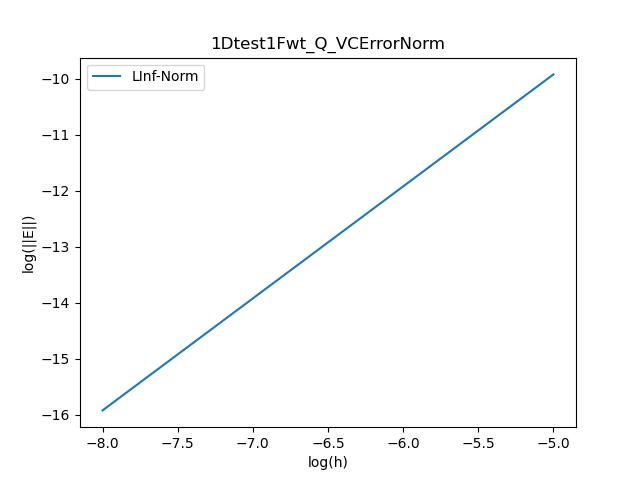
\includegraphics[width=0.35\linewidth]{1Dtest1Fwt_Q_VCErrorNorm.jpg}
        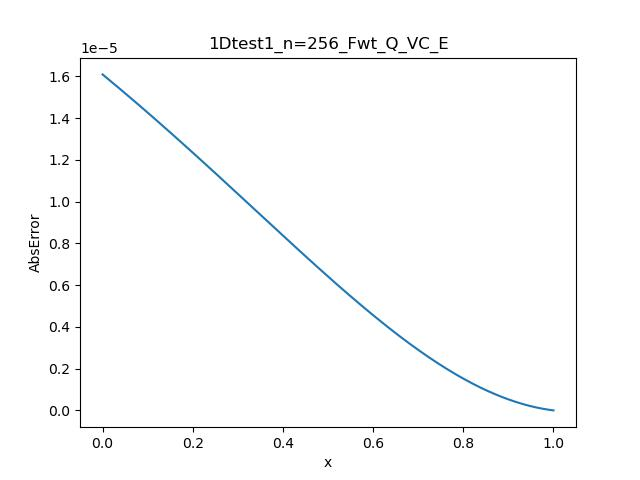
\includegraphics[width=0.35\linewidth]{1Dtest1_n=256_Fwt_Q_VC_E.jpg}
        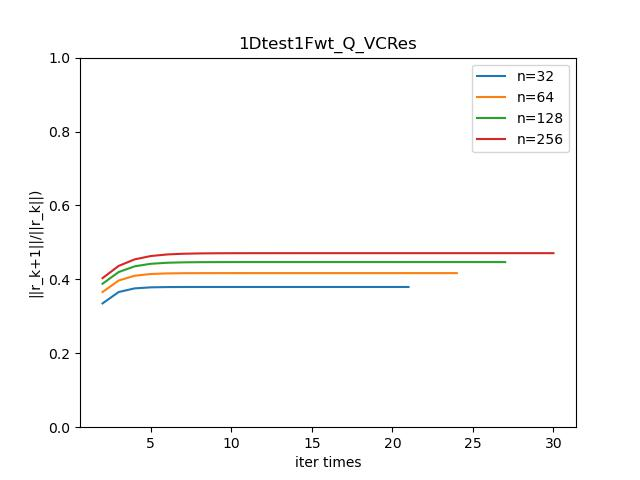
\includegraphics[width=0.35\linewidth]{1Dtest1Fwt_Q_VCRes.jpg}
        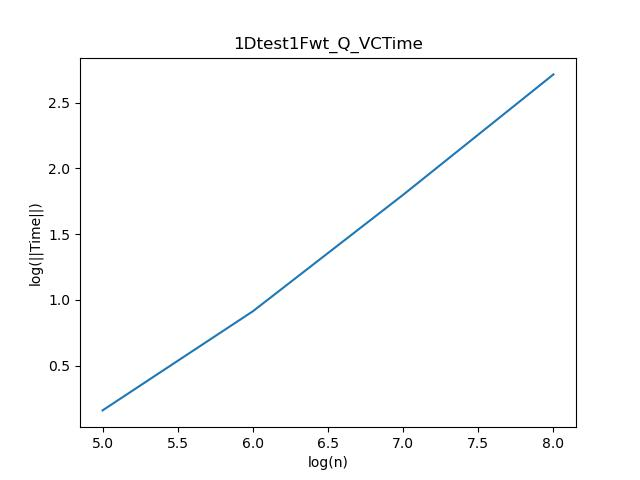
\includegraphics[width=0.35\linewidth]{1Dtest1Fwt_Q_VCTime.jpg}
    \end{figure}
    
    从图像可以判断收敛阶为2,残差的reduction rate 随网格变细从约为0.35变化到约为0.45, 时间复杂度为$O(n)$

    \item Injection, VC, Quadratic
    \begin{figure}[h]
        \centering
        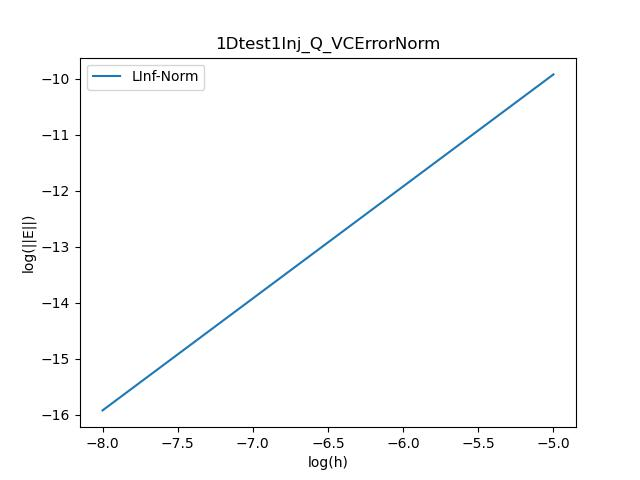
\includegraphics[width=0.35\linewidth]{1Dtest1Inj_Q_VCErrorNorm.jpg}
        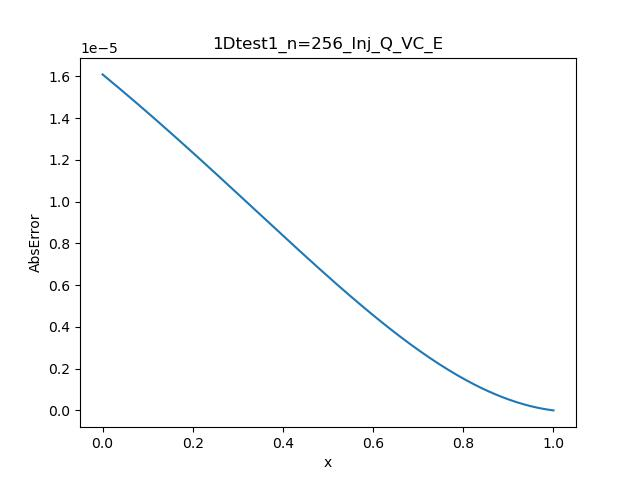
\includegraphics[width=0.35\linewidth]{1Dtest1_n=256_Inj_Q_VC_E.jpg}
        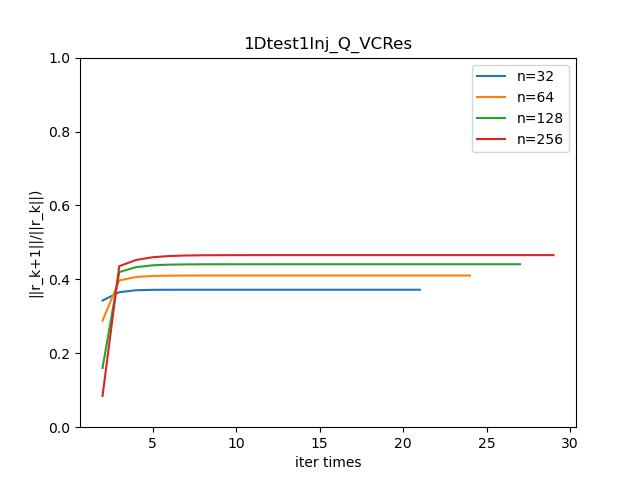
\includegraphics[width=0.35\linewidth]{1Dtest1Inj_Q_VCRes.jpg}
        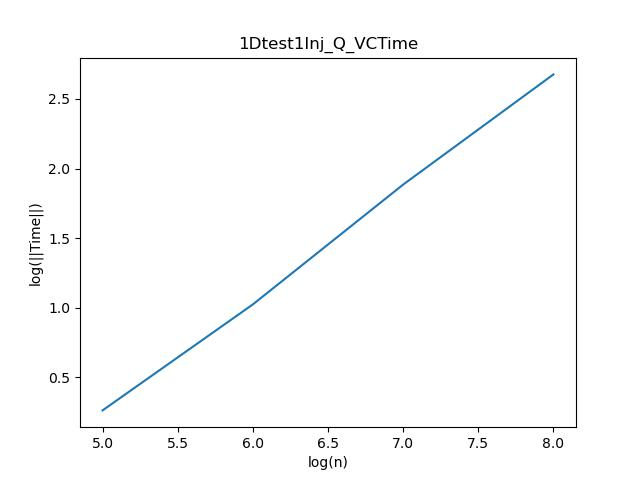
\includegraphics[width=0.35\linewidth]{1Dtest1Inj_Q_VCTime.jpg}
    \end{figure}
    
    从图像可以判断收敛阶为2,残差的reduction rate 随网格变细从约为0.35变化到约为0.45, 时间复杂度为$O(n)$
    \newpage
\end{itemize}

\subsubsection{1D: $u(x)=\sin(\pi x)$}
真实值:
\begin{figure}[h]
    \centering
    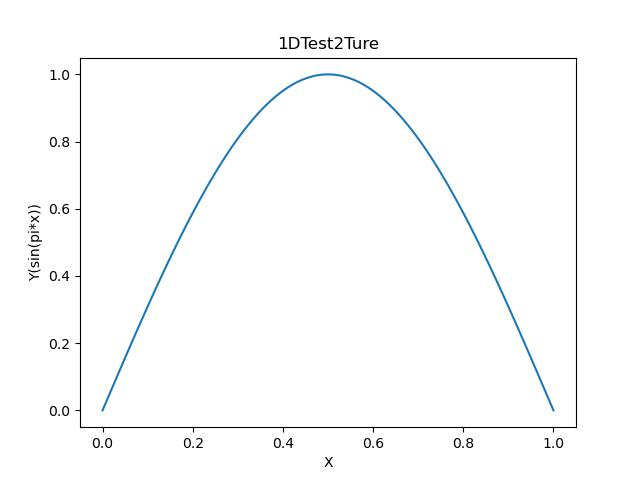
\includegraphics[width=0.7\linewidth]{1DTest2Ture.jpg}
\end{figure}

\begin{itemize}
    \item Full Weighting, FMG, Linear
    \begin{figure}[h]
        \centering
        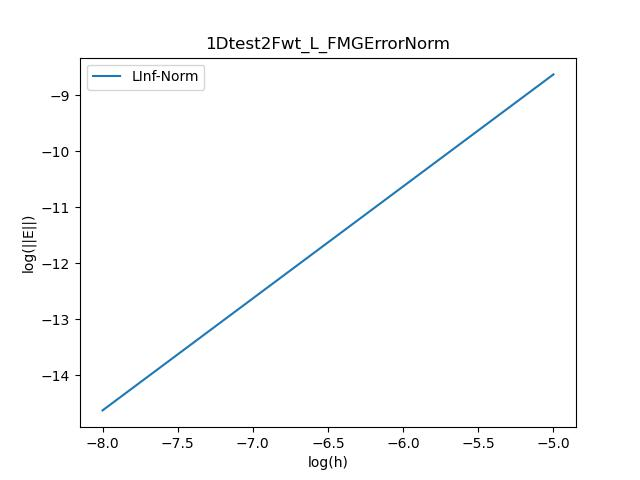
\includegraphics[width=0.35\linewidth]{1Dtest2Fwt_L_FMGErrorNorm.jpg}
        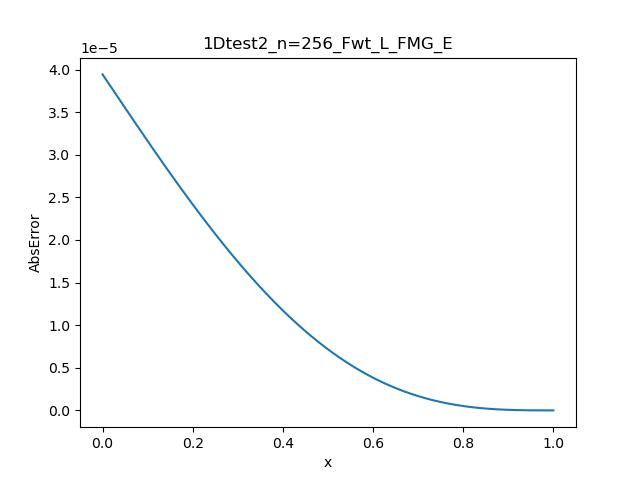
\includegraphics[width=0.35\linewidth]{1Dtest2_n=256_Fwt_L_FMG_E.jpg}
        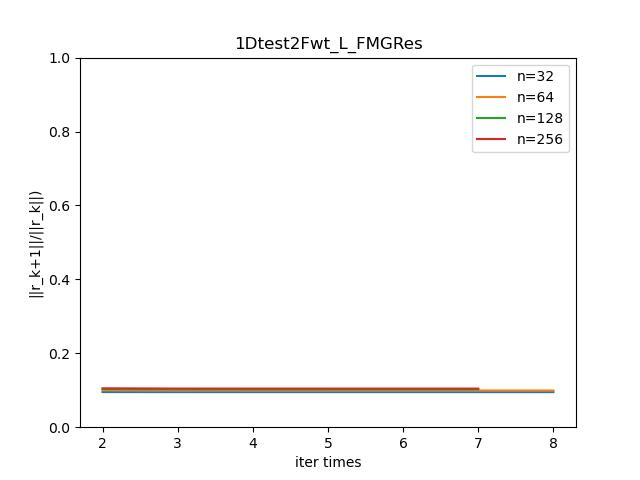
\includegraphics[width=0.35\linewidth]{1Dtest2Fwt_L_FMGRes.jpg}
        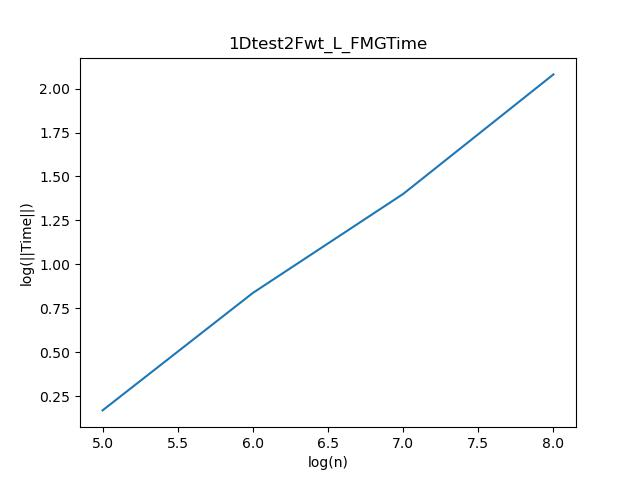
\includegraphics[width=0.35\linewidth]{1Dtest2Fwt_L_FMGTime.jpg}
    \end{figure}
    
    从图像可以判断收敛阶为2,残差的reduction rate 约为 0.1, 时间复杂度为$O(n)$
    \newpage
    \item Injection, FMG, Linear
    \begin{figure}[h]
        \centering
        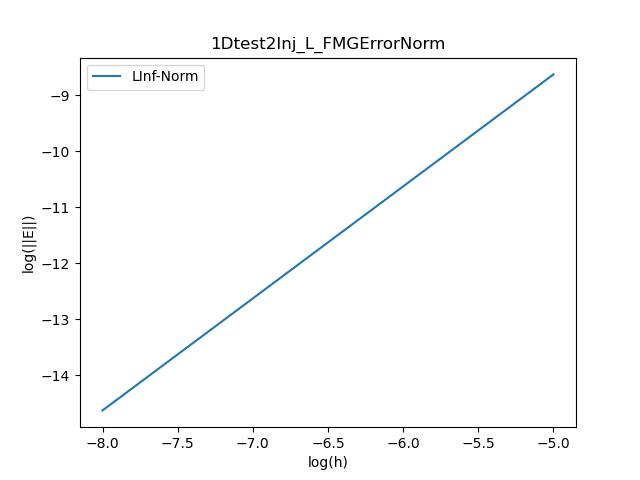
\includegraphics[width=0.35\linewidth]{1Dtest2Inj_L_FMGErrorNorm.jpg}
        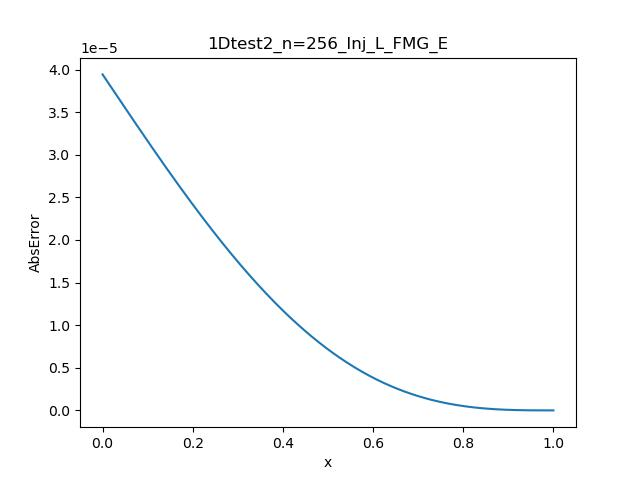
\includegraphics[width=0.35\linewidth]{1Dtest2_n=256_Inj_L_FMG_E.jpg}
        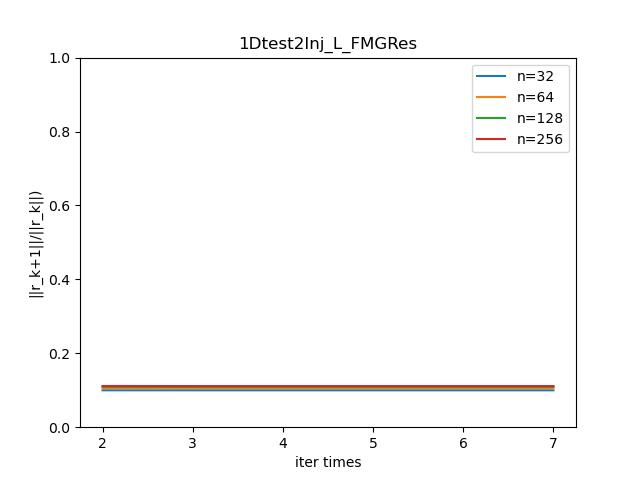
\includegraphics[width=0.35\linewidth]{1Dtest2Inj_L_FMGRes.jpg}
        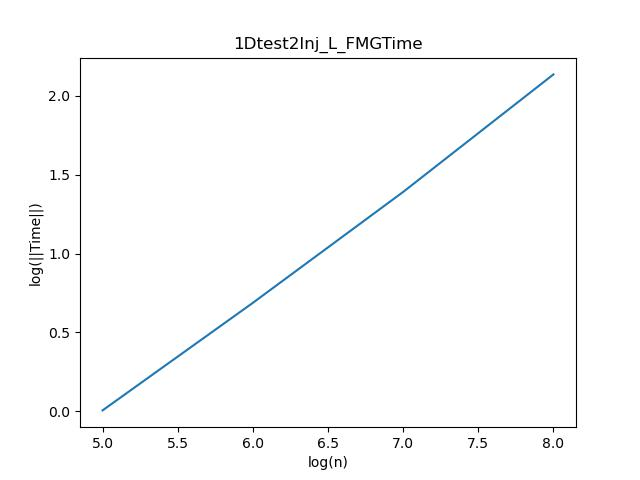
\includegraphics[width=0.35\linewidth]{1Dtest2Inj_L_FMGTime.jpg}
    \end{figure}
    
    从图像可以判断收敛阶为2,残差的reduction rate 约为 0.1, 时间复杂度为$O(n)$

    \item Full Weighting, VC, Linear
    \begin{figure}[h]
        \centering
        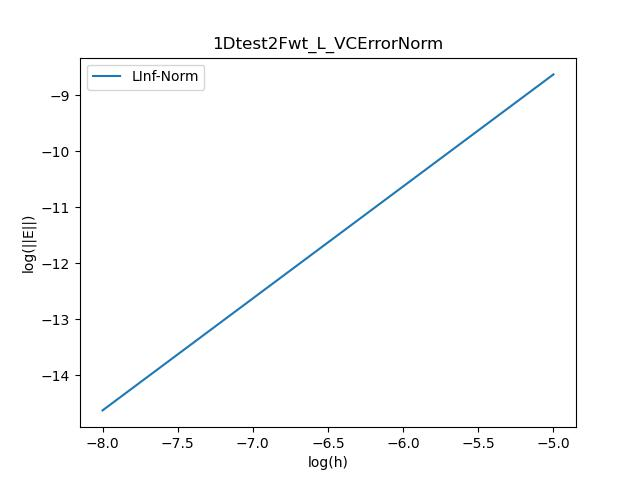
\includegraphics[width=0.35\linewidth]{1Dtest2Fwt_L_VCErrorNorm.jpg}
        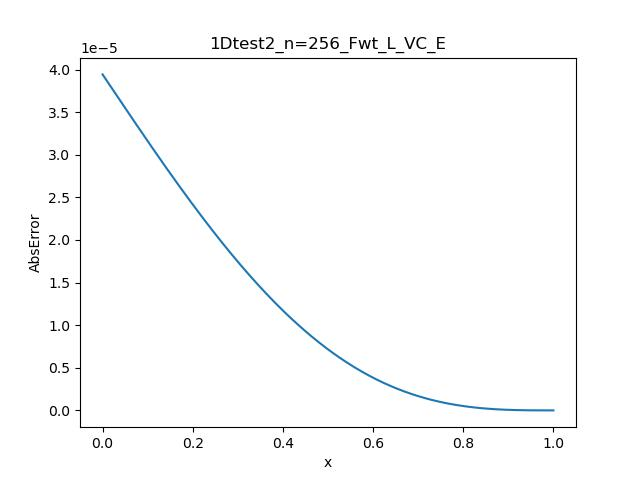
\includegraphics[width=0.35\linewidth]{1Dtest2_n=256_Fwt_L_VC_E.jpg}
        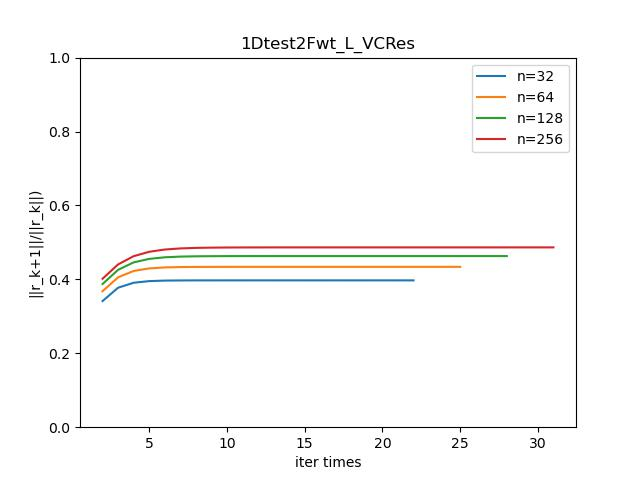
\includegraphics[width=0.35\linewidth]{1Dtest2Fwt_L_VCRes.jpg}
        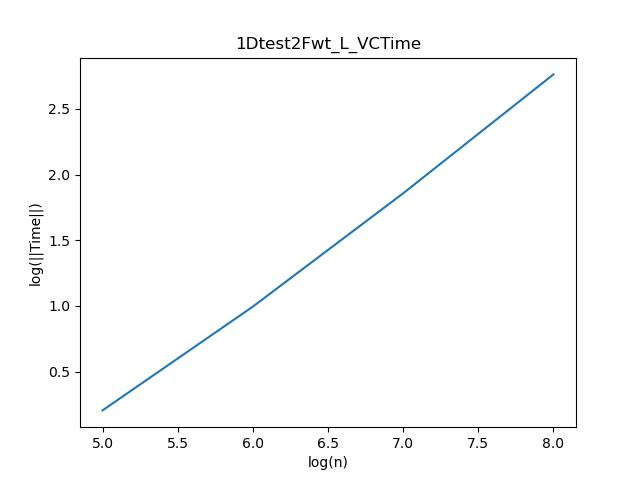
\includegraphics[width=0.35\linewidth]{1Dtest2Fwt_L_VCTime.jpg}
    \end{figure}
    
    从图像可以判断收敛阶为2,残差的reduction rate 随网格变细从约为0.35变化到约为0.45, 时间复杂度为$O(n)$
    \newpage
    \item Injection, VC, Linear
    \begin{figure}[h]
        \centering
        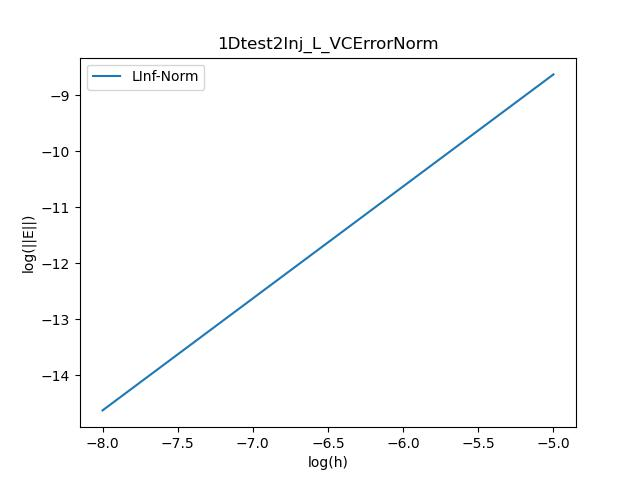
\includegraphics[width=0.35\linewidth]{1Dtest2Inj_L_VCErrorNorm.jpg}
        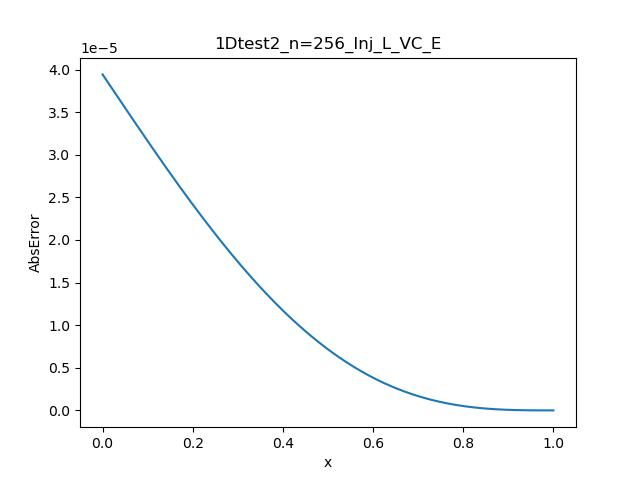
\includegraphics[width=0.35\linewidth]{1Dtest2_n=256_Inj_L_VC_E.jpg}
        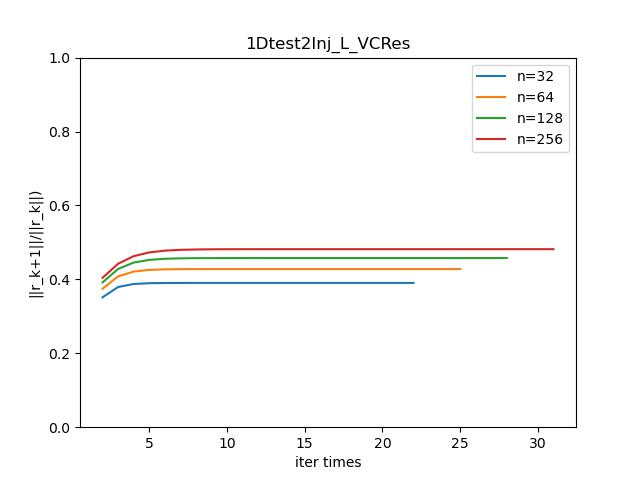
\includegraphics[width=0.35\linewidth]{1Dtest2Inj_L_VCRes.jpg}
        \includegraphics[width=0.35\linewidth]{1Dtest2Inj_L_VCTime.jpg}
    \end{figure}
    
    从图像可以判断收敛阶为2,残差的reduction rate 随网格变细从约为0.35变化到约为0.45, 时间复杂度为$O(n)$
    
    \item Full Weighting, FMG, Quadratic
    \begin{figure}[h]
        \centering
        \includegraphics[width=0.35\linewidth]{1Dtest2Fwt_Q_FMGErrorNorm.jpg}
        \includegraphics[width=0.35\linewidth]{1Dtest2_n=256_Fwt_Q_FMG_E.jpg}
        \includegraphics[width=0.35\linewidth]{1Dtest2Fwt_Q_FMGRes.jpg}
        \includegraphics[width=0.35\linewidth]{1Dtest2Fwt_Q_FMGTime.jpg}
    \end{figure}
    
    从图像可以判断收敛阶为2,残差的reduction rate 约为 0.1, 时间复杂度为$O(n)$
    \newpage
    \item Injection, FMG, Quadratic
    \begin{figure}[h]
        \centering
        \includegraphics[width=0.35\linewidth]{1Dtest2Inj_Q_FMGErrorNorm.jpg}
        \includegraphics[width=0.35\linewidth]{1Dtest2_n=256_Inj_Q_FMG_E.jpg}
        \includegraphics[width=0.35\linewidth]{1Dtest2Inj_Q_FMGRes.jpg}
        \includegraphics[width=0.35\linewidth]{1Dtest2Inj_Q_FMGTime.jpg}
    \end{figure}
    
    从图像可以判断收敛阶为2,残差的reduction rate 约为 0.1, 时间复杂度为$O(n)$
    

    \item Full Weighting, VC, Quadratic
    \begin{figure}[h]
        \centering
        \includegraphics[width=0.35\linewidth]{1Dtest2Fwt_Q_VCErrorNorm.jpg}
        \includegraphics[width=0.35\linewidth]{1Dtest2_n=256_Fwt_Q_VC_E.jpg}
        \includegraphics[width=0.35\linewidth]{1Dtest2Fwt_Q_VCRes.jpg}
        \includegraphics[width=0.35\linewidth]{1Dtest2Fwt_Q_VCTime.jpg}
    \end{figure}
    
    从图像可以判断收敛阶为2,残差的reduction rate 约为 随网格变细从约为0.35变化到约为0.45, 时间复杂度为$O(n)$
    \newpage
    \item Injection, VC, Quadratic
    \begin{figure}[h]
        \centering
        \includegraphics[width=0.35\linewidth]{1Dtest2Inj_Q_VCErrorNorm.jpg}
        \includegraphics[width=0.35\linewidth]{1Dtest2_n=256_Inj_Q_VC_E.jpg}
        \includegraphics[width=0.35\linewidth]{1Dtest2Inj_Q_VCRes.jpg}
        \includegraphics[width=0.35\linewidth]{1Dtest2Inj_Q_VCTime.jpg}
    \end{figure}
    
    从图像可以判断收敛阶为2,残差的reduction rate 约为 随网格变细从约为0.35变化到约为0.45, 时间复杂度为$O(n)$

\end{itemize}

\subsubsection{1D: $u(x)=x^3$}
真实值:
\begin{figure}[h]
    \centering
    \includegraphics[width=0.7\linewidth]{1DTest3Ture.jpg}
\end{figure}
\newpage
\begin{itemize}
    \item Full Weighting, FMG, Linear
    \begin{figure}[h]
        \centering
        \includegraphics[width=0.35\linewidth]{1Dtest3Fwt_L_FMGErrorNorm.jpg}
        \includegraphics[width=0.35\linewidth]{1Dtest3_n=256_Fwt_L_FMG_E.jpg}
        \includegraphics[width=0.35\linewidth]{1Dtest3Fwt_L_FMGRes.jpg}
        \includegraphics[width=0.35\linewidth]{1Dtest3Fwt_L_FMGTime.jpg}
    \end{figure}
    
    从图像可以判断收敛阶为2,残差的reduction rate 约为 0.1(即每迭代一次残差变为原先的0.1倍,下同), 时间复杂度为$O(n)$

    \item Injection, FMG, Linear
    \begin{figure}[h]
        \centering
        \includegraphics[width=0.35\linewidth]{1Dtest3Inj_L_FMGErrorNorm.jpg}
        \includegraphics[width=0.35\linewidth]{1Dtest3_n=256_Inj_L_FMG_E.jpg}
        \includegraphics[width=0.35\linewidth]{1Dtest3Inj_L_FMGRes.jpg}
        \includegraphics[width=0.35\linewidth]{1Dtest3Inj_L_FMGTime.jpg}
    \end{figure}
    
    从图像可以判断收敛阶为2,残差的reduction rate 约为 0.1, 时间复杂度为$O(n)$
    \newpage

    \item Full Weighting, VC, Linear
    \begin{figure}[h]
        \centering
        \includegraphics[width=0.35\linewidth]{1Dtest3Fwt_L_VCErrorNorm.jpg}
        \includegraphics[width=0.35\linewidth]{1Dtest3_n=256_Fwt_L_VC_E.jpg}
        \includegraphics[width=0.35\linewidth]{1Dtest3Fwt_L_VCRes.jpg}
        \includegraphics[width=0.35\linewidth]{1Dtest3Fwt_L_VCTime.jpg}
    \end{figure}
    
    从图像可以判断收敛阶为2,残差的reduction rate 约为 随网格变细从约为0.35变化到约为0.45, 时间复杂度为$O(n)$

    \item Injection, VC, Linear
    \begin{figure}[h]
        \centering
        \includegraphics[width=0.35\linewidth]{1Dtest3Inj_L_VCErrorNorm.jpg}
        \includegraphics[width=0.35\linewidth]{1Dtest3_n=256_Inj_L_VC_E.jpg}
        \includegraphics[width=0.35\linewidth]{1Dtest3Inj_L_VCRes.jpg}
        \includegraphics[width=0.35\linewidth]{1Dtest3Inj_L_VCTime.jpg}
    \end{figure}
    
    从图像可以判断收敛阶为2,残差的reduction rate 约为 随网格变细从约为0.35变化到约为0.45, 时间复杂度为$O(n)$
    \newpage
    \item Full Weighting, FMG, Quadratic
    \begin{figure}[h]
        \centering
        \includegraphics[width=0.35\linewidth]{1Dtest3Fwt_Q_FMGErrorNorm.jpg}
        \includegraphics[width=0.35\linewidth]{1Dtest3_n=256_Fwt_Q_FMG_E.jpg}
        \includegraphics[width=0.35\linewidth]{1Dtest3Fwt_Q_FMGRes.jpg}
        \includegraphics[width=0.35\linewidth]{1Dtest3Fwt_Q_FMGTime.jpg}
    \end{figure}
    
    从图像可以判断收敛阶为2,残差的reduction rate 约为 0.1, 时间复杂度为$O(n)$

    \item Injection, FMG, Quadratic
    \begin{figure}[h]
        \centering
        \includegraphics[width=0.35\linewidth]{1Dtest3Inj_Q_FMGErrorNorm.jpg}
        \includegraphics[width=0.35\linewidth]{1Dtest3_n=256_Inj_Q_FMG_E.jpg}
        \includegraphics[width=0.35\linewidth]{1Dtest3Inj_Q_FMGRes.jpg}
        \includegraphics[width=0.35\linewidth]{1Dtest3Inj_Q_FMGTime.jpg}
    \end{figure}
    
    从图像可以判断收敛阶为2,残差的reduction rate 约为 0.1, 时间复杂度为$O(n)$
    \newpage

    \item Full Weighting, VC, Quadratic
    \begin{figure}[h]
        \centering
        \includegraphics[width=0.35\linewidth]{1Dtest3Fwt_Q_VCErrorNorm.jpg}
        \includegraphics[width=0.35\linewidth]{1Dtest3_n=256_Fwt_Q_VC_E.jpg}
        \includegraphics[width=0.35\linewidth]{1Dtest3Fwt_Q_VCRes.jpg}
        \includegraphics[width=0.35\linewidth]{1Dtest3Fwt_Q_VCTime.jpg}
    \end{figure}
    
    从图像可以判断收敛阶为2,残差的reduction rate 约为 随网格变细从约为0.35变化到约为0.45, 时间复杂度为$O(n)$

    \item Injection, VC, Quadratic
    \begin{figure}[h]
        \centering
        \includegraphics[width=0.35\linewidth]{1Dtest3Inj_Q_VCErrorNorm.jpg}
        \includegraphics[width=0.35\linewidth]{1Dtest3_n=256_Inj_Q_VC_E.jpg}
        \includegraphics[width=0.35\linewidth]{1Dtest3Inj_Q_VCRes.jpg}
        \includegraphics[width=0.35\linewidth]{1Dtest3Inj_Q_VCTime.jpg}
    \end{figure}
    
    从图像可以判断收敛阶为2,残差的reduction rate 约为 随网格变细从约为0.35变化到约为0.45, 时间复杂度为$O(n)$
    \newpage
\end{itemize}

\subsubsection{2D: $u(x,y)=e^{y+\sin(x)}$}
真实值:
\begin{figure}[h]
    \centering
    \includegraphics[width=0.7\linewidth]{2DTest1True.jpg}
\end{figure}

\begin{itemize}
    \item Full Weighting, FMG, Linear
    \begin{figure}[h]
        \centering
        \includegraphics[width=0.35\linewidth]{2Dtest1Fwt_L_FMGErrorNorm.jpg}
        \includegraphics[width=0.35\linewidth]{2Dtest1_n=256_Fwt_L_FMG_E.jpg}
        \includegraphics[width=0.35\linewidth]{2Dtest1Fwt_L_FMGRes.jpg}
        \includegraphics[width=0.35\linewidth]{2Dtest1Fwt_L_FMGTime.jpg}
    \end{figure}
    
    从图像可以判断收敛阶为2,残差的reduction rate 随网格变细从约为0.35变化到约为0.5, 时间复杂度为$O(n^2)$
    \newpage
    \item Injection, FMG, Linear
    \begin{figure}[h]
        \centering
        \includegraphics[width=0.35\linewidth]{2Dtest1Inj_L_FMGErrorNorm.jpg}
        \includegraphics[width=0.35\linewidth]{2Dtest1_n=256_Inj_L_FMG_E.jpg}
        \includegraphics[width=0.35\linewidth]{2Dtest1Inj_L_FMGRes.jpg}
        \includegraphics[width=0.35\linewidth]{2Dtest1Inj_L_FMGTime.jpg}
    \end{figure}
    
    从图像可以判断收敛阶为2,残差的reduction rate 随网格变细从约为0.35变化到约为0.5, 时间复杂度为$O(n^2)$

    \item Full Weighting, VC, Linear
    \begin{figure}[h]
        \centering
        \includegraphics[width=0.35\linewidth]{2Dtest1Fwt_L_VCErrorNorm.jpg}
        \includegraphics[width=0.35\linewidth]{2Dtest1_n=256_Fwt_L_VC_E.jpg}
        \includegraphics[width=0.35\linewidth]{2Dtest1Fwt_L_VCRes.jpg}
        \includegraphics[width=0.35\linewidth]{2Dtest1Fwt_L_VCTime.jpg}
    \end{figure}
    
    从图像可以判断收敛阶为2,残差的reduction rate 随网格变细从约为0.6变化到约为0.8, 时间复杂度为$O(n^2)$
    \newpage
    \item Injection, VC, Linear
    \begin{figure}[h]
        \centering
        \includegraphics[width=0.35\linewidth]{2Dtest1Inj_L_VCErrorNorm.jpg}
        \includegraphics[width=0.35\linewidth]{2Dtest1_n=256_Inj_L_VC_E.jpg}
        \includegraphics[width=0.35\linewidth]{2Dtest1Inj_L_VCRes.jpg}
        \includegraphics[width=0.35\linewidth]{2Dtest1Inj_L_VCTime.jpg}
    \end{figure}
    
    从图像可以判断收敛阶为2,残差的reduction rate 随网格变细从约为0.6变化到约为0.8, 时间复杂度为$O(n^2)$
\end{itemize}

\subsubsection{2D: $u(x,y)=\sin(\pi x)\sin(\pi y)$}
真实值:
\begin{figure}[h]
    \centering
    \includegraphics[width=0.7\linewidth]{2DTest2True.jpg}
\end{figure}
\newpage
\begin{itemize}
    \item Full Weighting, FMG, Linear
    \begin{figure}[h]
        \centering
        \includegraphics[width=0.35\linewidth]{2Dtest2Fwt_L_FMGErrorNorm.jpg}
        \includegraphics[width=0.35\linewidth]{2Dtest2_n=256_Fwt_L_FMG_E.jpg}
        \includegraphics[width=0.35\linewidth]{2Dtest2Fwt_L_FMGRes.jpg}
        \includegraphics[width=0.35\linewidth]{2Dtest2Fwt_L_FMGTime.jpg}
    \end{figure}
    
    从图像可以判断收敛阶为2,残差的reduction rate 随网格变细从约为0.35变化到约为0.5, 时间复杂度为$O(n^2)$
    
    \item Injection, FMG, Linear
    \begin{figure}[h]
        \centering
        \includegraphics[width=0.35\linewidth]{2Dtest2Inj_L_FMGErrorNorm.jpg}
        \includegraphics[width=0.35\linewidth]{2Dtest2_n=256_Inj_L_FMG_E.jpg}
        \includegraphics[width=0.35\linewidth]{2Dtest2Inj_L_FMGRes.jpg}
        \includegraphics[width=0.35\linewidth]{2Dtest2Inj_L_FMGTime.jpg}
    \end{figure}
    
    从图像可以判断收敛阶为2,残差的reduction rate 随网格变细从约为0.35变化到约为0.5, 时间复杂度为$O(n^2)$
    \newpage
    \item Full Weighting, VC, Linear
    \begin{figure}[h]
        \centering
        \includegraphics[width=0.35\linewidth]{2Dtest2Fwt_L_VCErrorNorm.jpg}
        \includegraphics[width=0.35\linewidth]{2Dtest2_n=256_Fwt_L_VC_E.jpg}
        \includegraphics[width=0.35\linewidth]{2Dtest2Fwt_L_VCRes.jpg}
        \includegraphics[width=0.35\linewidth]{2Dtest2Fwt_L_VCTime.jpg}
    \end{figure}
    
    从图像可以判断收敛阶为2,残差的reduction rate 随网格变细从约为0.6变化到约为0.8, 时间复杂度为$O(n^2)$
    
    \item Injection, VC, Linear
    \begin{figure}[h]
        \centering
        \includegraphics[width=0.35\linewidth]{2Dtest2Inj_L_VCErrorNorm.jpg}
        \includegraphics[width=0.35\linewidth]{2Dtest2_n=256_Inj_L_VC_E.jpg}
        \includegraphics[width=0.35\linewidth]{2Dtest2Inj_L_VCRes.jpg}
        \includegraphics[width=0.35\linewidth]{2Dtest2Inj_L_VCTime.jpg}
    \end{figure}
    
    从图像可以判断收敛阶为2,残差的reduction rate 随网格变细从约为0.6变化到约为0.8, 时间复杂度为$O(n^2)$
    \newpage
\end{itemize}

\subsubsection{2D: $u(x,y)=x^3+y^3$}
真实值:
\begin{figure}[h]
    \centering
    \includegraphics[width=0.7\linewidth]{2DTest3True.jpg}
\end{figure}

\begin{itemize}
    \item Full Weighting, FMG, Linear
    \begin{figure}[h]
        \centering
        \includegraphics[width=0.35\linewidth]{2Dtest3Fwt_L_FMGErrorNorm.jpg}
        \includegraphics[width=0.35\linewidth]{2Dtest3_n=256_Fwt_L_FMG_E.jpg}
        \includegraphics[width=0.35\linewidth]{2Dtest3Fwt_L_FMGRes.jpg}
        \includegraphics[width=0.35\linewidth]{2Dtest3Fwt_L_FMGTime.jpg}
    \end{figure}
    
    从图像可以判断收敛阶为2,残差的reduction rate 随网格变细从约为0.35变化到约为0.5, 时间复杂度为$O(n^2)$
    \newpage
    \item Injection, FMG, Linear
    \begin{figure}[h]
        \centering
        \includegraphics[width=0.35\linewidth]{2Dtest3Inj_L_FMGErrorNorm.jpg}
        \includegraphics[width=0.35\linewidth]{2Dtest3_n=256_Inj_L_FMG_E.jpg}
        \includegraphics[width=0.35\linewidth]{2Dtest3Inj_L_FMGRes.jpg}
        \includegraphics[width=0.35\linewidth]{2Dtest3Inj_L_FMGTime.jpg}
    \end{figure}
    
    从图像可以判断收敛阶为2,残差的reduction rate 随网格变细从约为0.35变化到约为0.5, 时间复杂度为$O(n^2)$

    \item Full Weighting, VC, Linear
    \begin{figure}[h]
        \centering
        \includegraphics[width=0.35\linewidth]{2Dtest3Fwt_L_VCErrorNorm.jpg}
        \includegraphics[width=0.35\linewidth]{2Dtest3_n=256_Fwt_L_VC_E.jpg}
        \includegraphics[width=0.35\linewidth]{2Dtest3Fwt_L_VCRes.jpg}
        \includegraphics[width=0.35\linewidth]{2Dtest3Fwt_L_VCTime.jpg}
    \end{figure}
    
    从图像可以判断收敛阶为2,残差的reduction rate 随网格变细从约为0.6变化到约为0.8, 时间复杂度为$O(n^2)$
    \newpage
    \item Injection, VC, Linear
    \begin{figure}[h]
        \centering
        \includegraphics[width=0.35\linewidth]{2Dtest3Inj_L_VCErrorNorm.jpg}
        \includegraphics[width=0.35\linewidth]{2Dtest3_n=256_Inj_L_VC_E.jpg}
        \includegraphics[width=0.35\linewidth]{2Dtest3Inj_L_VCRes.jpg}
        \includegraphics[width=0.35\linewidth]{2Dtest3Inj_L_VCTime.jpg}
    \end{figure}
    
    从图像可以判断收敛阶为2,残差的reduction rate 随网格变细从约为0.6变化到约为0.8, 时间复杂度为$O(n^2)$
\end{itemize}

\subsubsection{与LU分解的耗时对比}
这里选取的测试函数为2Dtest3:$u(x,y)=x^3+y^3$,网格大小为$n=64$,
测试结果如下

\begin{center} 
    \begin{tabular}{ccc}
        \toprule
        FMG & VC & LU-factorization  \\
        \midrule
        80ms & 125ms  & 12637ms \\
        \bottomrule
    \end{tabular}
\end{center}

两者相差了近160(100)倍,从实验结果看多重网格实现了$O(N)$的时间复杂度,而LU分解为$O(N^3)$的时间复杂度,其中$N=n^D$,所以差距将会随着n的变大急剧变大。

\subsubsection{精度测试}
实验结果如下
\begin{verbatim}
    eps     1DResidual  2DResidual  1Diter  2Diter  
    1e-09   8.05379e-10 5.04632e-10 10      33      
    1e-10   8.4127e-11  4.79984e-11 11      36      
    1e-11   8.7876e-12  4.56539e-12 12      39      
    1e-12   9.17921e-13 9.51289e-13 13      41      
    1e-13   9.58827e-14 9.04824e-14 14      44      
    1e-14   1.04619e-15 8.60628e-15 16      47      
    1e-15   1.09281e-16 8.18592e-16 17      50      
    2.2e-16 1.09281e-16 1.7057e-16  17      52  
\end{verbatim}

将预设精度不段减小至$2.2\times 10^{-16}$,始终能达到预设精度,大概是机器精度还挺高的
\subsection{总结分析}
从数值结果看对于一维和二维的多重网格都实现了二阶精度的收敛,且都达到了$O(N),\ N=n^D$的时间复杂度,并且从各个函数的误差分布图像可以看出误差分布只与求解的方程已经边界条件有关,不同的restriction、prolongation和cycle不会影响误差分布。
并且对比一维的测试结果可以发现二次插值相比线性插值对于误差的减小没有肉眼可见的提升。此外可以发现随着网格不断变细,残差的reduction rate 相应变低(数值上变大),在二维的测试中可以明显的观测到,一维情况下可能是数据量的变化太小,不能看到明显的变低,可以勉强看出所有测试都是$n=256$时最低。
并且在一维和二维情形上FMG相比VC有巨大的提升。
\end{document}